\clearpage
\chapter{Melody Writing}
\label{sec:melody-writing}

\subsection*{What you can do after this chapter}
\begin{itemize}
  \item Recognise a motive in a melody and tell a motive from a whole phrase.
  \item Grow a motive into a four-bar phrase with repetition, sequence, inversion, retrograde, and augmentation or diminution.
  \item Write a four-bar question and answer: the question ends on the dominant or a non-tonic tone, and the answer returns to tonic.
  \item Place chord tones and tension tones with intent, then lay the melody out in Yeban's piano roll.
\end{itemize}

\subsection{Motive: the smallest memorable unit}

A motive is a short musical idea that can be remembered and reused, usually two to five notes or one striking rhythm. It does not need a complete meaning, but it needs a recognisable shape: contour, rhythm, accent, or register, with at least one of them standing out.

Take C--D--E--G: the contour rises low--middle--high--higher, and the rhythm might be long--short--short--long. When D--E--F--A arrives, you hear ``the same sentence, moved up.'' When C--B--A--F arrives, you hear ``the direction is reversed, but the skeleton is still there.'' That is a motive's identifying power.

A motive is not ``any four notes.'' If there is no repeatable contour or rhythm, the next phrase cannot recognise it. When writing a motive, ask what you want remembered: a leap, a rhythm, or a timbre. Protect that one thing; the rest may change.

\subsection{Phrase and question--answer: how four bars hold together}

A phrase is a melody that can stand as a sentence; in pop writing it is often four or eight bars. The most common four-bar shape is two bars of question and two bars of answer:

\begin{itemize}
  \item \textbf{Antecedent (question)}: states the motive and ends on the dominant, a non-tonic tone, or an unresolved high note, so the ear waits.
  \item \textbf{Consequent (answer)}: picks up the motive and ends on the tonic or tonic function, so the ear lands.
\end{itemize}

A question does not have to sound like a literal question. It is simply unclosed: it may stop on G4 (dominant), E4 (third), or a tension tone. The answer need not repeat the question exactly; it can change the ending, rhythm, or register, as long as ``unfinished'' becomes ``finished.''

A common approach is to share the first two bars of the motive and diverge only in the last two. The ear first recognises ``there it is again,'' then hears ``this time it lands.'' If question and answer are identical, it is usually repetition, not a question--answer pair; if the answer uses entirely new material, it can sound like a different sentence.


\begin{center}
\begin{minipage}{0.92\linewidth}
\centering
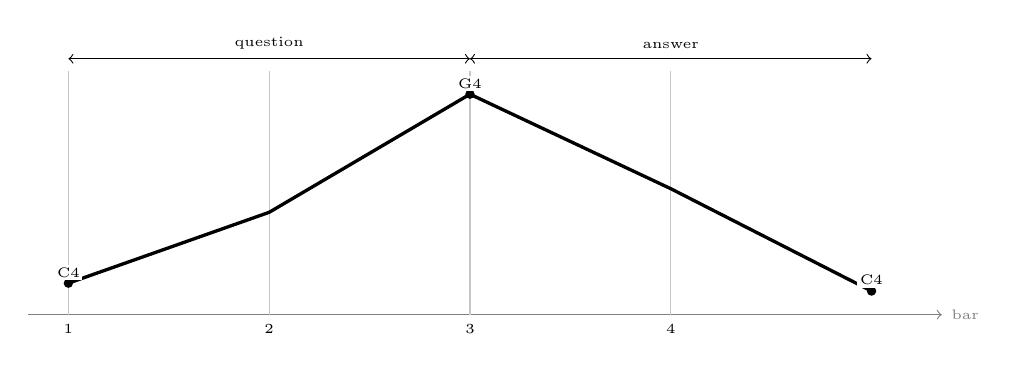
\begin{tikzpicture}[x=2.55cm,y=1.0cm,font=\scriptsize]
  \draw[->,gray] (-0.2,-0.2) -- (4.35,-0.2) node[right,font=\tiny]{bar};
  \foreach \x/\lab in {0/1,1/2,2/3,3/4} {
    \draw[gray!45] (\x,-0.2) -- (\x,2.9);
    \node[below,font=\tiny] at (\x,-0.2) {\lab};
  }
  \draw[very thick] (0,0.2) -- (1,1.1) -- (2,2.6) -- (3,1.4) -- (4,0.1);
  \foreach \x/\y/\n in {0/0.2/C4,2/2.6/G4,4/0.1/C4} {
    \fill (\x,\y) circle (1.7pt);
    \node[above=1pt,font=\tiny,fill=white,inner sep=1pt] at (\x,\y) {\n};
  }
  \draw[<->] (0,3.05) -- (2,3.05) node[midway,above,font=\tiny]{question};
  \draw[<->] (2,3.05) -- (4,3.05) node[midway,above,font=\tiny]{answer};
\end{tikzpicture}

Figure 7-2. Tension and landing points across four bars. The question rises to G4 in bar 2; the answer returns to C4 in bar 4. The curve shows relative tension, not exact pitch.
\end{minipage}
\end{center}

\subsection{Repetition, sequence, and variation: growing the motive}

A motive grows by more than exact repetition. Six devices are most useful:

\begin{center}
\small
\begin{tabular}{p{0.16\linewidth}p{0.26\linewidth}p{0.44\linewidth}}
\toprule
Device & What to do & Effect \\
\midrule
Repetition & Play it again unchanged & emphasis, memorability \\
Sequence & Move it to another pitch, keeping contour and rhythm & forward motion, ``same sentence in another voice'' \\
Inversion & Mirror it around a pitch axis & familiar but strange; good for a turn \\
Retrograde & Play it backwards from the last note & a sense of review or closing \\
Augmentation / diminution & Double or halve all durations & same motive slower or faster; mood changes \\
Ornamentation & Add passing or neighbour tones between structural notes & smoother, but do not bury the skeleton \\
\bottomrule
\end{tabular}

Table 7-1. Six ways to vary a motive. Use one or two at a time; too many and the original is lost.
\end{center}

Sequence is the easiest device to overuse: three or four rising sequences in a row sound like a staircase, and listeners tire quickly. Usually one or two sequences are enough; the third should change direction, rhythm, or simply stop. Inversion and retrograde should not be used merely to sound ``advanced''; the further they move from the original contour, the more the surrounding context must explain the relationship.

\begin{center}
\begin{minipage}{0.86\linewidth}
\centering
\begin{tikzpicture}[x=1.55cm,y=0.55cm,xshift=0.55cm,font=\scriptsize]
  % original: C D E G
  \foreach \x/\y/\n in {0/6/C,1/6.9/D,2/7.8/E,3/9.4/G} {
    \fill (\x,\y) circle (1.6pt);
    \node[above=1pt] at (\x,\y) {\n};
  }
  \draw (0,6) -- (1,6.9) -- (2,7.8) -- (3,9.4);
  
  % sequence: D E F A
  \foreach \x/\y/\n in {0/3/D,1/3.9/E,2/4.8/F,3/6.4/A} {
    \fill (\x,\y) circle (1.6pt);
    \node[above=1pt] at (\x,\y) {\n};
  }
  \draw (0,3) -- (1,3.9) -- (2,4.8) -- (3,6.4);
  
  % inversion: C B A F
  \foreach \x/\y/\n in {0/0/C,1/-0.9/B,2/-1.8/A,3/-3.4/F} {
    \fill (\x,\y) circle (1.6pt);
    \node[below=1pt] at (\x,\y) {\n};
  }
  \draw (0,0) -- (1,-0.9) -- (2,-1.8) -- (3,-3.4);
  \end{tikzpicture}

Figure 7-1. Three contours of the same motive, from top to bottom: original, sequence, inversion. The original rises, the sequence moves the whole shape up, and the inversion reverses direction; this is a contour sketch, not staff notation.
\end{minipage}
\end{center}

\subsection{Melody and harmony: when to land on a chord tone, when to use a tension tone}

A melody is not ``play every chord tone in order.'' It moves between stable and unstable: land on chord tones on strong beats, use passing and neighbour tones on weak beats to keep the line smooth, and use tension tones for colour.

\begin{center}
\begin{minipage}{\linewidth}
\centering
\small
\begin{tabular}{p{0.16\linewidth}p{0.28\linewidth}p{0.42\linewidth}}
\toprule
Type & Example over a C chord & Use \\
\midrule
Chord tone & C, E, G & strong beats, phrase endings, landing points; stable \\
Passing tone & D (between C and E) & weak beat, moves by step to the next chord tone \\
Neighbour tone & F (above E) & leaves E and returns to E; a small wave \\
Appoggiatura & F on a strong beat, resolving to E & grabs the ear with tension, then settles \\
Tension tone & A (6), D (9), B (major 7) & colour and suspense; needs context to resolve or justify \\
\bottomrule
\end{tabular}

Table 7-2. Melody notes against a C major triad. A tension tone is not a ``wrong note,'' but it needs resolution or stylistic support.
\end{minipage}
\end{center}

The safest order is ``write the melody first, harmonise second.'' If you fix the chords first and fill every chord tone, the melody easily becomes an arpeggio exercise. In practice, hum four bars first, then ask: which chord tone does the strong beat land on? Does the phrase end on tonic or dominant? If the strong beats keep hitting tension tones, change the melody or the chords; do not pretend you cannot hear it.

\textbf{Chord-lane boundary:} Yeban's chord lane is fixed five-block demo data and does not follow the project's actual chords. It can only serve as an i--VI--iv--V reference; it is not ``the current project harmony'' for setting a melody. To harmonise, write the chords yourself in the roll, or judge by ear.

\subsection{Rhythmic motive: same pitches, different rhythm, another sentence}

A rhythmic motive is a memory point independent of exact pitch. Change the four notes C--D--E--G from long--short--short--long to short--short--short--long, and listeners hear two different musical sentences even though the pitches are identical.

\begin{center}
\small
\begin{tabular}{p{0.14\linewidth}p{0.30\linewidth}p{0.42\linewidth}}
\toprule
Rhythm & In 4/4 & Effect \\
\midrule
Even & one note per beat, or one per half beat & steady, forward, good for statement \\
Dotted & long plus short, ``long--short'' & springy, a little swing \\
Syncopated & accents on weak beats or off-beats & strong push, common in pop and funk \\
Triplet & three notes in one beat & flowing, dense; good for transition or ornament \\
\bottomrule
\end{tabular}

Table 7-3. Four basic rhythmic motives. Clap the pulse first, then write it into the roll.
\end{center}

When writing a rhythmic motive, clap or speak the accents first, then decide which notes fall on strong beats. Syncopation is not ``move a note half a beat later at random'': it needs a stable pulse around it, or it just sounds late. Triplets should not run for too many bars; after density, return to even rhythm so the ear can rest.

\subsection{How to do it in Yeban}

\begin{enumerate}
  \item Create a 4/4 project, select a MIDI instrument track, and open the piano roll (P/F7).
  \item In bar 1, write a four-beat motive: C4, D4, E4, G4, with a long--short--short--long rhythm. Write only this bar first and press Space to hear the contour.
  \item Use Copy Clip (Ctrl+C) and Paste Clip (Ctrl+V) to copy bar 1 into bar 2; select the four notes in bar 2 and move each up by two rows to get the D--E--F--A sequence.
  \item In bars 3--4, write the answer: catch the motive in the first two beats and end on C4. The question's second bar should end on G4, not C.
  \item Turn on the metronome and loop with Space or Loop Playback (C). Listen repeatedly: at the end of the question, does the ear still want more? At the end of the answer, has it really landed?
  \item Make two variations: first change only rhythm (double the first note), then change only contour (turn the rise into an inversion); keep the chord tones and the final tonic.
\end{enumerate}

\screenshot{piano-roll-four-bar-question-answer}{Four-bar question and answer}{Four-bar question and answer}

\textbf{Scope note:} Yeban currently has no automatic melody generation, motive detection, phrase analysis, or question/answer judgement; these depend on your ear and manual note edits. The chord lane is fixed five-block demo data and does not follow project chords; to harmonise for real, write chords or an audio track in the roll. The app will not decide whether a note is a ``tension tone'' or a ``wrong note''; that depends on context and style.

\subsection{Exercises}

\begin{enumerate}
  \item Using C--D--E--G as the original, write a sequence up a second, an inversion around C, and a retrograde.
  \par\noindent Answer: sequence D--E--F--A; inversion C--B--A--F; retrograde G--E--D--C.
  \item Write a four-bar question and answer: the question ends on G4 in two bars, the answer returns to C4 in two bars. Explain why you closed it that way.
  \par\noindent Answer: not unique. A valid answer ends the question on a non-tonic tone and the answer on C4, and the answer audibly responds to the motive.
  \item Over a C major triad, what roles do C, E, G, D, F, A, and B play?
  \par\noindent Answer: C/E/G are chord tones; D can be a passing tone or the 9th; F can be a neighbour, appoggiatura, or tension tone; A is a 6th tension; B is a major-7th tension or leading tone.
  \item With the same four notes, which is more likely to preserve the motive's identity: changing only rhythm or changing only pitch? Why?
  \par\noindent Answer: rhythm is usually more recognisable; contour also matters, and changing both at once loses the original most easily.
  \item In Yeban, copy the four-beat motive from bar 1 to bar 2 and make it a sequence. Which menu or shortcut did you use?
  \par\noindent Answer: Copy Clip Ctrl+C and Paste Clip Ctrl+V; select the four notes in bar 2 and move them up two rows.
\end{enumerate}

\subsection{Help topic map}

\begin{center}
\small
\begin{tabular}{p{0.30\linewidth}p{0.42\linewidth}p{0.20\linewidth}}
\toprule
Section & In-app help anchor & Note \\
\midrule
Motive & \texttt{music-theory-motive} & concept \\
Phrase and question--answer & \texttt{music-theory-phrase} & four-bar shape \\
Repetition and sequence & \texttt{music-theory-sequence} & Table 7-1 \\
Melody and harmony & \texttt{music-theory-melody-harmony} & Table 7-2 \\
Rhythmic motive & \texttt{music-theory-rhythm-motive} & Table 7-3 \\
How to in Yeban & \texttt{music-theory-piano-roll-melody} & operation \\
Exercises & \texttt{music-theory-ch7-practice} & answers at chapter end \\
\bottomrule
\end{tabular}
\end{center}
